% RLC-Serienschwingkreis - Phasenkurve von w/w0 mit Q=1,2,3,4,1000 (phi = phi_U - phi_I)
\def\R{10}%     10 Ohm
\def\L{10e-3}%  10 mH
\def\C{10e-6}%  10 uF
\def\Zk{31.623}% Zk = sqrt(L/C) = 31.623 Ohm
% w0 = 1/sqrt(LC) = 3162.278 Hz
% Güte Q = Zk/R -> R = Zk/Q
\def\Zk{31.623}
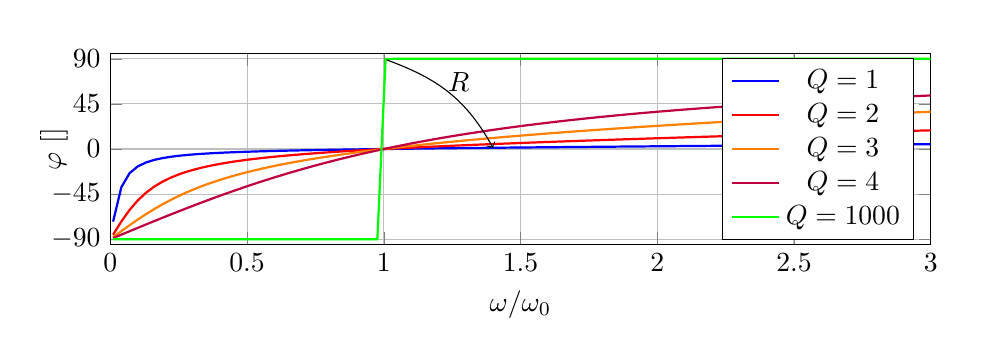
\begin{tikzpicture}[x=1cm,y=1cm]
    \draw[draw=none] (-1.05,-1) rectangle (10.75,2.75); % boundbox (not matching width and height, don't know why) % set draw=black (debug) or draw=none (final)
    \begin{axis}[
        xlabel={$\omega/\omega_0$},
        ylabel={$\varphi\ [\degree]$},
        ylabel style={yshift=-0.45cm},
        xmin=0, xmax=3,
        ymin=-95, ymax=95,
        width=12cm,
        height=4cm,
        samples=100,
        grid=both,
        xtick={0, 0.5, 1, 1.5, 2, 2.5, 3},
        ytick={-90,-45,0,45,90},
    ] 
    % Phi = atan(Im/Re) = atan(Zk * (w/w0 - w0/w) / R) = atan( Q * (w/w0 - w0/w)
    \addplot[domain=0.01:3, mark=$Q=1$, thick, color=blue]     {atan((1*(x-1/x))/(31.62))};% R=31.62 Güte 1
    \addplot[domain=0.01:3, mark=$Q=2$, thick, color=red]      {atan((2*(x-1/x))/(15.81))};% R=15.81 Güte 2
    \addplot[domain=0.01:3, mark=$Q=3$, thick, color=orange]   {atan((3*(x-1/x))/(10.54))};% R=10.54 Güte 3
    \addplot[domain=0.01:3, mark=$Q=4$, thick, color=purple]   {atan((4*(x-1/x))/(7.91))};% R=7.91 Güte 4
    \addplot[domain=0.01:3, mark=$Q=1000$, thick, color=green] {atan((1000*(x-1/x))/(0.032))};% R=0.032 Güte 1000
    \addlegendentry{$Q=1$}
    \addlegendentry{$Q=2$}
    \addlegendentry{$Q=3$}
    \addlegendentry{$Q=4$}
    \addlegendentry{$Q=1000$}
    % R Pfeil
    \draw [->](axis cs:1.01, 89) .. controls (axis cs:1.2, 70) and (axis cs:1.3, 50) .. (axis cs:1.4, 1)
    node[pos=0.6, above]{$R$};
    \end{axis}
\end{tikzpicture}